\section{连续性校正}

\subsection{使用原因}
由中心极限定理,独立同分布的随机变量序列$X_i,\;i=1,2\dots,n$的和$\sum\limits_{i=1}^{n}X_i$将在随机变量个数$n\to+\infty$时服从正态分布,因此,在某些情况下,我们可以利用正态分布CDF(Cumulative Distribution Function)值来近似一些难以计算的离散型随机变量(Discrete Variable)的CDF值。

\begin{figure}[htbp] 
	\centering 
	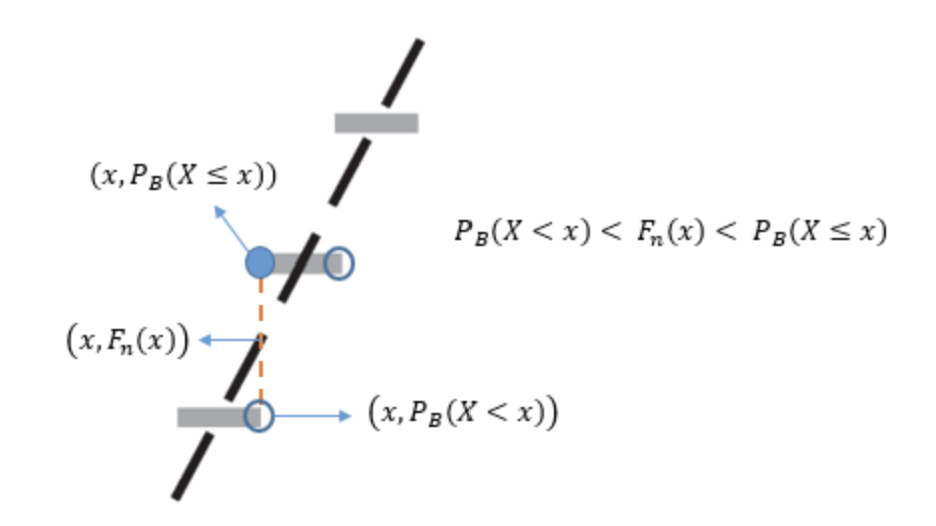
\includegraphics{probability-theory/chapter4/CDF-of-c-and-d-variables.png} 
	\caption{连续型、离散型随机变量CDF图} 
\end{figure}

\hspace{2em}对于离散型随机变量,常出现$P(X<x)\ne P(X\leqslant x)$,而对于连续型随机变量(Continuous Variable),二者的值是相等的,因此,CDF值的近似将出现以下问题:
\begin{enumerate}
	\item 使用正态分布CDF值近似$P(X\leqslant x)$时近似值偏小。
	\item 使用正态分布CDF值近似$P(X< x)$时近似值偏大。
\end{enumerate}
\hspace{2em}而我们会想要得到一个一致的近似,即对于以上两个近似,结果总是一致地偏大或偏小,这样利于分析。

\subsection{具体方法}
\begin{itemize}
	\item 根据近似的分布选择一个$\alpha\in (-1,1)$,一般选择$\pm\frac{1}{2}$。
	\item 使用正态分布CDF值$F(\frac{x+\alpha-\mu}{\sigma})$近似$P(X< x)$与$P(X\leqslant x)$。
\end{itemize}